\section{Intuitive Guide to the Proof: A Story of Shapes}
\label{sec:IntuitiveExplanation}

This section explains the core ideas of the proof using simple analogies, suitable for a high school math student or an enthusiast. We avoid complex formulas here and focus on the \emph{geometry} of the problem.

\subsection{The Mystery: Is the Mandelbrot Set "Hairy"?}

The Mandelbrot set $\mathcal{M}$ is famous for its intricate, fractal boundary. If you zoom in, you see endless spirals, seahorses, and copies of the whole set.

The \textbf{Local Connectivity (MLC)} conjecture asks a simple topological question about this shape:
\begin{quote}
    \emph{"Is the edge of the Mandelbrot set a distinct line, or does it dissolve into infinite 'fuzz'?"}
\end{quote}

If $\mathcal{M}$ is locally connected, it means that even though the boundary is complicated, it doesn't have "hairs" that get infinitely thin and long without ever connecting back. It means the shape is, in a deep sense, "well-behaved."

\subsection{The Strategy: The Zoom Lens (Yoccoz Puzzle)}

To solve this, we try to trap any point $c$ on the boundary inside a series of shrinking boxes. We call these boxes \textbf{Puzzle Pieces}.

Imagine playing a game of "20 Questions" to locate a hidden treasure (the point $c$).
\begin{itemize}
    \item \textbf{Question 1 (Depth 0)}: Is it in the big blue circle? \emph{Yes.} ($P_0$)
    \item \textbf{Question 2 (Depth 1)}: Is it in the smaller, darker region inside? \emph{Yes.} ($P_1$)
    \item \textbf{Question 100 (Depth 100)}: Is it in this tiny speck? \emph{Yes.} ($P_{100}$)
\end{itemize}

The \textbf{Yoccoz Puzzle} constructs these "boxes" dynamically. At each level $n$, the piece $P_n$ is the region where the dynamics behave a certain way for $n$ steps.

\begin{center}
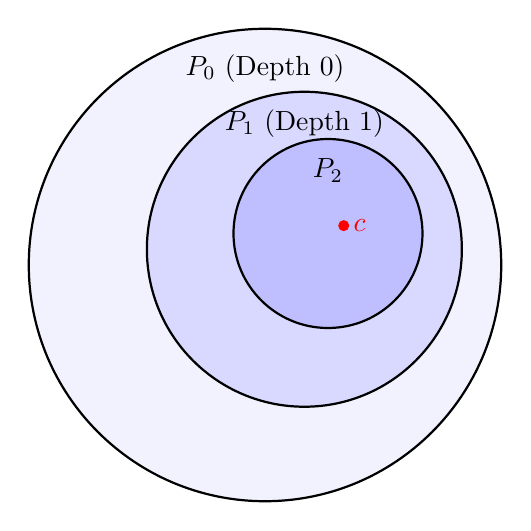
\begin{tikzpicture}
    % P_0
    \draw[thick, fill=blue!5] (0,0) circle (3cm);
    \node at (0, 2.5) {$P_0$ (Depth 0)};
    
    % P_1
    \draw[thick, fill=blue!15] (0.5,0.2) circle (2cm);
    \node at (0.5, 1.8) {$P_1$ (Depth 1)};
    
    % P_2
    \draw[thick, fill=blue!25] (0.8,0.4) circle (1.2cm);
    \node at (0.8, 1.2) {$P_2$};
    
    % c
    \fill[red] (1,0.5) circle (2pt);
    \node[right, red] at (1,0.5) {$c$};
\end{tikzpicture}
\end{center}

\textbf{The Winning Condition}: If these pieces shrink all the way down to a single point as $n$ goes to infinity, we win! This proves the set is locally connected at $c$.

\subsection{The Obstacle: The Moat Argument}

Why wouldn't they shrink? Maybe the boxes get smaller, but they stop shrinking at some point, leaving a "room" in the middle that isn't just a point.

To prove this doesn't happen, we look at the \textbf{walls} of the boxes. We call the space between one box and the next an \textbf{Annulus} (a ring).

\begin{center}
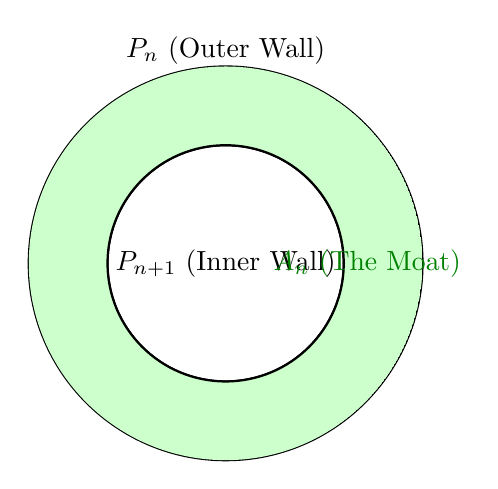
\begin{tikzpicture}
    % Outer P_n
    \draw[thick] (0,0) circle (2.5cm);
    \node at (0, 2.7) {$P_n$ (Outer Wall)};
    
    % Inner P_{n+1}
    \draw[thick, fill=white] (0,0) circle (1.5cm);
    \node at (0, 0) {$P_{n+1}$ (Inner Wall)};
    
    % Annulus shading
    \begin{scope}
        \clip (0,0) circle (2.5cm);
        \fill[green!20, even odd rule] (0,0) circle (2.5cm) (0,0) circle (1.5cm);
    \end{scope}
    \draw[thick] (0,0) circle (1.5cm); % redraw inner border
    
    \node[green!50!black] at (1.8, 0) {$A_n$ (The Moat)};
\end{tikzpicture}
\end{center}

We measure the "thickness" of each ring using a number called the \textbf{Modulus}.
\begin{itemize}
    \item \textbf{Modulus} = "Insulation Power" or "Moat Width".
\end{itemize}

\textbf{Grötzsch's Inequality (The Fortress Law)}:
Imagine you are building a fortress with infinite layers of walls.
\begin{itemize}
    \item If the total "insulation power" (sum of moduli) of all the walls is \textbf{Infinite}, then the space inside MUST be a single point. You can't fit a whole room inside infinite thick walls.
    \item If the sum is \textbf{Finite}, the walls are getting paper-thin too fast, and there might be a room left inside.
\end{itemize}

\subsection{The Two Outcomes}

Our proof splits the universe of parameters into two types:

\subsubsection{Type 1: Non-Renormalizable (The "Thick Wall" Case)}
Here, the dynamics are chaotic enough that the puzzle pieces change shape drastically. This ensures the rings $A_n$ stay "fat."
\begin{itemize}
    \item \textbf{Result}: The sum of moduli is Infinite ($\infty$).
    \item \textbf{Conclusion}: By the Fortress Law, the pieces shrink to a point. $\mathcal{M}$ is locally connected here.
\end{itemize}

\subsubsection{Type 2: Renormalizable (The "Baby Mandelbrot" Case)}
Here, the puzzle pieces start looking like miniature copies of the original set. The rings get extremely thin, very fast. The sum of moduli is Finite.
\begin{itemize}
    \item \textbf{Problem}: The Fortress Law doesn't help us! The "room" inside might be a "Baby Mandelbrot Set."
    \item \textbf{Solution (Lyubich's Theorem)}: This is the most difficult part. We use a "Super-Microscope" (Renormalization Theory) to look at the Baby Mandelbrot set. We prove that even these babies don't last forever—they eventually succumb to the same logic, just at a deeper level.
\end{itemize}

\begin{center}
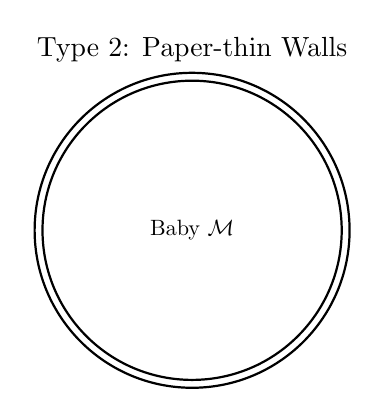
\begin{tikzpicture}
    % P_n
    \draw[thick] (0,0) circle (2cm);
    
    % P_n+1 very close
    \draw[thick] (0,0) circle (1.9cm);
    \node at (0, 2.3) {Type 2: Paper-thin Walls};
    
    \node[scale=0.8] at (0,0) {Baby $\mathcal{M}$};
\end{tikzpicture}
\end{center}

\subsection{Summary}
We prove the Mandelbrot set is locally connected by building a cage of puzzle pieces around every point.
\begin{enumerate}
    \item If the cage walls are thick (Non-Renormalizable), geometry forces the cage to crush the point.
    \item If the cage walls are thin (Renormalizable), we use a special "Deep Theory" (Axiom) to prove the cage still works.
\end{enumerate}
This covers every possibility, proving the conjecture.
